\documentclass{article}
\usepackage{tikz}

\begin{document}

\begin{figure}[h]
    \centering
    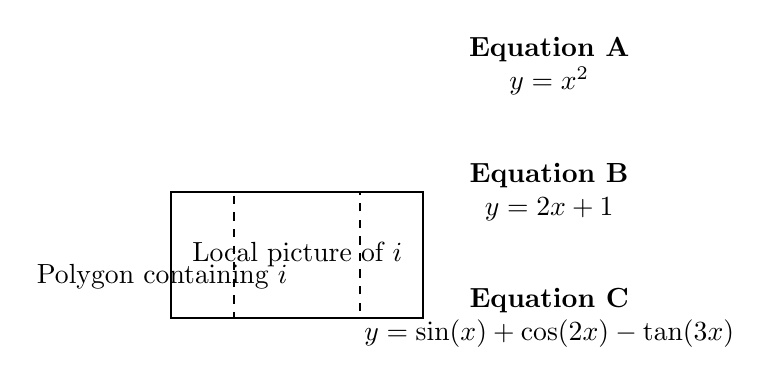
\begin{tikzpicture}[scale=0.8]

        % Draw the local picture of i on the surface
        \draw[thick] (-2,-1) rectangle (2,1);
        \node at (0,0) {Local picture of $i$};

        % Draw the polygon containing i
        \draw[dashed, thick] (-1,-1) -- (1,-1) -- (1,1) -- (-1,1) -- cycle;
        \node at (0,0) [below left] {Polygon containing $i$};

        % Position for the equations
        \coordinate (eq1) at (4,3);
        \coordinate (eq2) at (4,1);
        \coordinate (eq3) at (4,-1);

        % Equation 1: Simple equation
        \node at (eq1) [align=center] {
            \textbf{Equation A} \\
            $y = x^2$
        };

        % Equation 2: Simple equation
        \node at (eq2) [align=center] {
            \textbf{Equation B} \\
            $y = 2x + 1$
        };

        % Equation 3: Complex equation
        \node at (eq3) [align=center] {
            \textbf{Equation C} \\
            $y = \sin(x) + \cos(2x) - \tan(3x)$
        };

    \end{tikzpicture}
    \caption{Local picture of $i$ on the surface, polygon containing $i$, and equations representing the coordinates of a curve.}
    \label{fig:curve-coordinates}
\end{figure}

\end{document}